\chapter{Evaluation}
\label{chap:evaluation}

% compare:
% - mono (no best fuzzer for sample programs)
% - multi vs single (more communication is better if multi > single)
% - coop vs union (test coop efficacy)

This chapter presents an evaluation of four different fuzzers and our
implementation of the \acf{CFF} as described in \autoref{sec:system-impl}; the
implementation uses the same four fuzzers in order to draw meaningful comparison
results. In \autoref{sec:eval-mono} we compare the results, in terms of
coverage, of running fuzzers without cooperation; \autoref{sec:eval-coop}
presents results of running the same fuzzers with cooperation. Lastly
\autoref{sec:eval-crashes} presents an evaluation of cooperative fuzzing in
terms of crashes found.

\paragraph{Choice of Fuzzers}

For the choice of fuzzers we decided to use \aflfast, \fairfuzz, \honggfuzz\ and
\vuzzer. The first two provide two different implementations of the
state-of-the-art \ac{CGF}, \afl; we argue that two different implementation of
the same core algorithm may yield different results. \honggfuzz\ is chosen as it
provides different means to extract feedback from the \sut, possibly resulting
in a different feedback signal (given the same input) compared to other methods
(\eg\ \afl\ uses QEMU). Lastly, \vuzzer\ provides with an evolutionary fuzzer
which uses static and lightweight program analysis; because of this, \ac{CFF}
uses the congestion control mechanism to interact with \vuzzer. All fuzzers were
run with the default parameters and configuration, with the exception of those
required to correctly interface with the \sut.  Moreover, as already mentioned
in \autoref{sec:driver-impl}, all these fuzzers (besides \honggfuzz) support a
file system based synchronization mechanism to periodically import new test
cases; for \honggfuzz, we use an extended version that mimics AFL's
synchronization component.

\paragraph{Experimental Infrastructure}

Experiments were run on a 64-bit machine with $8$ cores (running at $3.4$GHz),
with $16$GB of RAM, running Ubuntu 16.04. Because of a limitation of \vuzzer\
implementation, we had to run it inside a virtual machine hosting Ubuntu 14.04.
To allow communication with its driver running on the host machine, we used a
shared folder; this allowed us to reuse the \texttt{inotify} infrastructure as
if the fuzzer was running locally. Finally, we disable \ac{ASLR} before fuzzing
and when running the crash triaging script; in the latter, we also limit the
available address space to simulate the same environment of the fuzzer that
found the crash.

\paragraph{Testing Targets}

We chose a set of programs that are widely used both in practice and literature:

\begin{description}
    \item[\djpeg] uses the popular \texttt{libjpeg-turbo} (version 1.5.1) and
        has been used for the evaluation of \fairfuzz\ and \vuzzer;
    \item[\objdump] is a component of the suite \texttt{binutils} (version 2.28)
        which has also been tested by \aflfast\ and \fairfuzz; we test it with
        the command line option \texttt{-d}, which provides a disassembler;
    \item[\tiffpdf] from the popular \texttt{libtiff} (version 4.0.9), parses a
        TIFF image and converts it to a PDF\@; we use it without command line
        arguments;
    \item[\listswf] from the popular \texttt{libming} (version 0.4.8), parses a
        file in SWF format; we use it without command line arguments.
\end{description}

Moreover, as \vuzzer\ requires a minimum set of seed inputs to work properly,
we randomly chose the minimum required by \vuzzer\ from test samples provided
with each \sut; these inputs were used to also seed other fuzzers.

As an additional information, we report on the number of basic block and
functions found by static analysis via Radare\footnote{\url{https://rada.re/}}
in \autoref{tab:eval-bbs}.

\begin{table}[h]
    \centering%
    \begin{tabular}{l c c}
        \textbf{\sut} & \textbf{basic blocks} & \textbf{functions} \\
        \bottomrule%
        \djpeg& $6187$ & $366$ \\
        \objdump& $43211$ & $2220$ \\
        \tiffpdf& $11129$ & $791$ \\
        \listswf& $3349$ & $446$
    \end{tabular}
    \caption{Number of basic blocks and functions for the chosen targets.}
    \label{tab:eval-bbs}
\end{table}

\section{Single Fuzzer Evaluation}
\label{sec:eval-mono}

In this section we present an evaluation of the chosen fuzzers, without any
cooperation. We ran each fuzzer independently for $24$ hours on each of the
targets, except for \listswf\ which ran for $6$ hours. \autoref{tab:eval-mono}
reports the arithmetic mean and the $95\%$ confidence intervals for the number
of unique basic block transitions as computed by Intel \ac{BTS} over five
rounds. The coverage values are aggregated over time intervals of one minute.

\begin{table}[h]
    \centering%
    \small%
    \begin{adjustbox}{tabular=l*{4}c,center}
        \textbf{\sut} & \textbf{\aflfast} & \textbf{\fairfuzz} &
            \textbf{\honggfuzz} & \textbf{\vuzzer} \\
        \bottomrule%
        \djpeg& $3739.4 \pm 113.831$ & $4043.2 \pm 103.838$ &
            \hicell$4112.8 \pm 39.5483$ & $2801 \pm 53.5514$ \\
        \objdump& $4762.6 \pm 23.3693$ & \hicell$5067 \pm 62.6832$ &
            $4132.4 \pm 104.8$ & $3162.2 \pm 138.462$ \\
        \tiffpdf& \hicell$8971.2 \pm 152.865$ & $8813.8 \pm 146.756$ &
            $5260.2 \pm 148.591$ & $3616 \pm 34.6427$ \\
        \listswf& $6831.6 \pm 2615.24$ & \hicell$8586.8 \pm 87.7467$ &
            $6345.6 \pm 2358.52$ & $5048.2 \pm 90.3928$
    \end{adjustbox}
    \caption{Mean coverage with $95\%$ confidence intervals for single fuzzers.
    Highlighted is the best for the given program.}
    \label{tab:eval-mono}
\end{table}

By looking at the table, as well as at \autoref{fig:eval-mono}, which presents
the evolution of coverage over time, it is easy to see how no fuzzer is
decisively better than the others across all tested programs. This validates,
although for a small sample of programs and fuzzers, our intuition based on the
no free lunch theorem, for which there is no fuzzer that performs better than
all others across all possible test programs.

\begin{figure}[h]
    \centering%
    \begin{adjustbox}{center}
        \subfloat[\djpeg]{%
            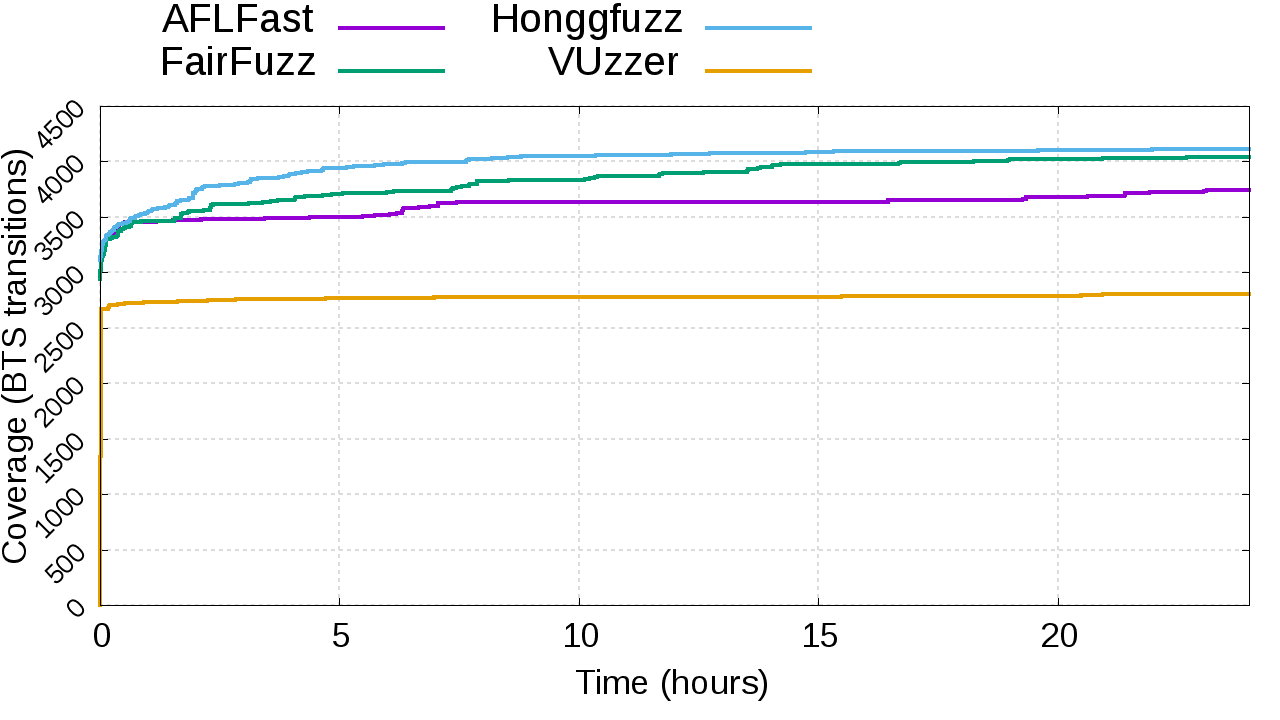
\includegraphics[width=.65\textwidth]{figures/mono-djpeg}
            \label{fig:eval-mono-djpeg}
        }
        \subfloat[\objdump]{%
            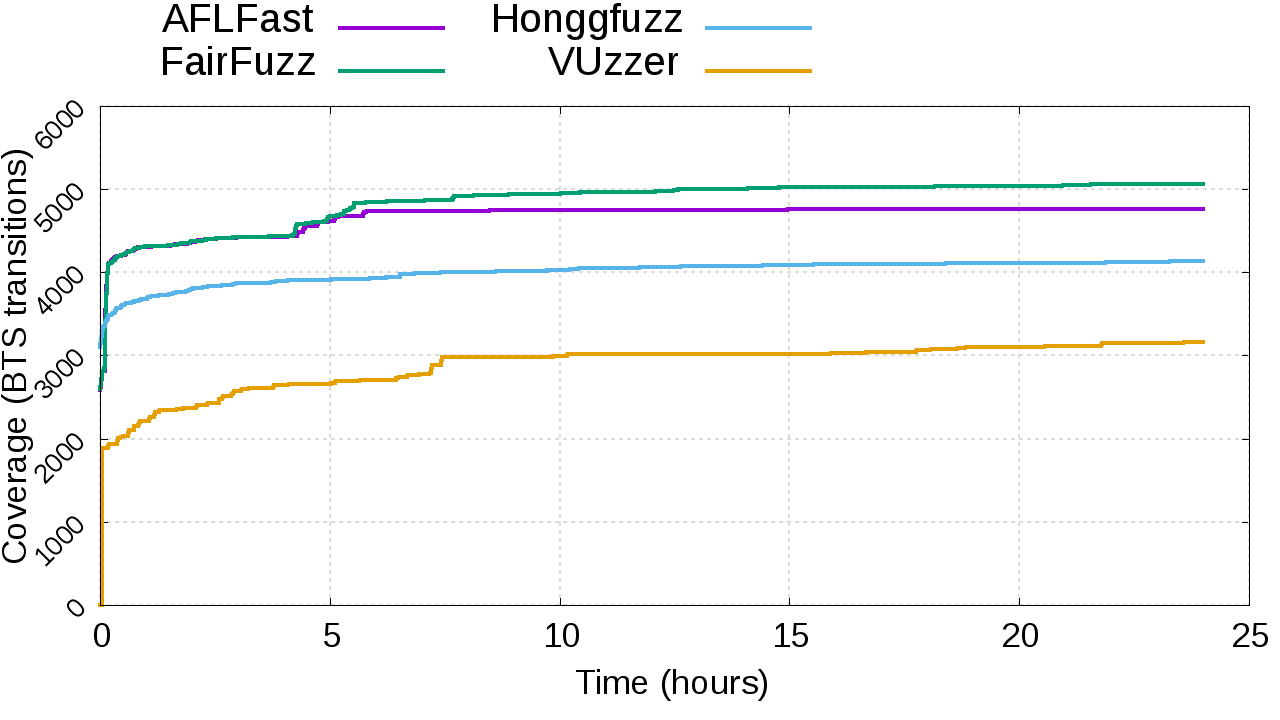
\includegraphics[width=.65\textwidth]{figures/mono-objdump}
            \label{fig:eval-mono-objdump}
        }
    \end{adjustbox}
    \begin{adjustbox}{center}
        \subfloat[\tiffpdf]{%
            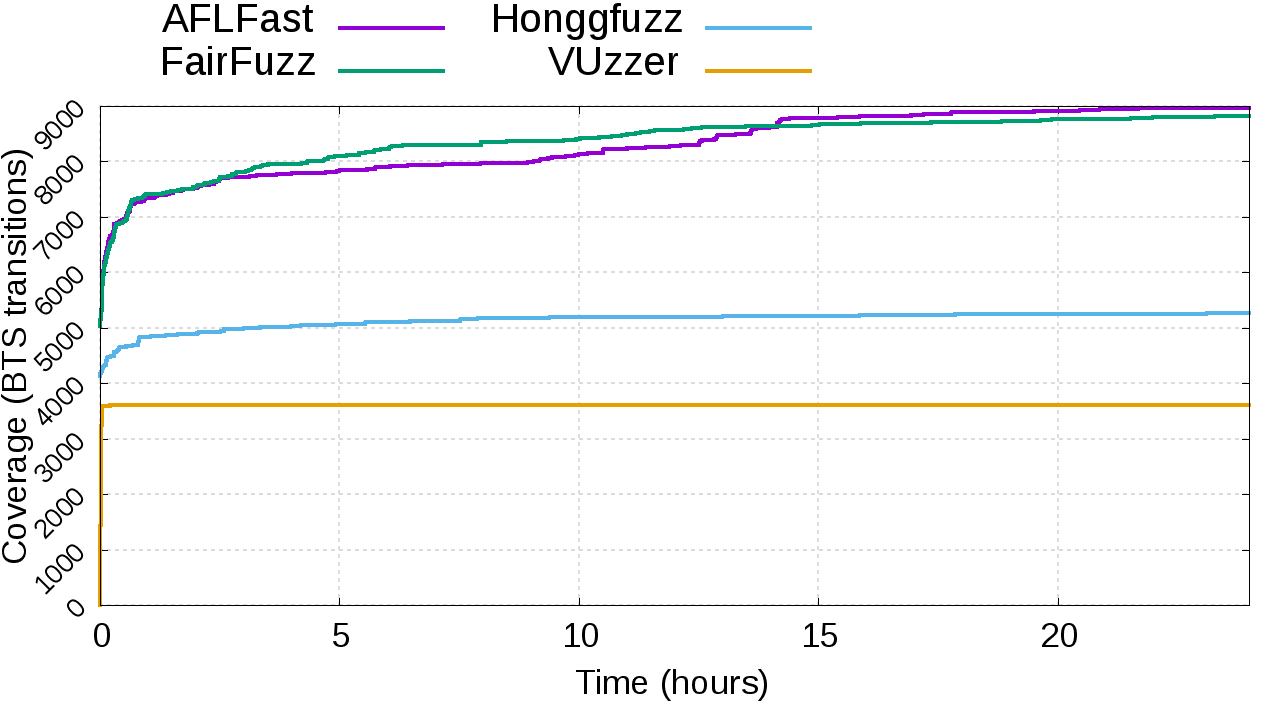
\includegraphics[width=.65\textwidth]{figures/mono-tiff2pdf}
            \label{fig:eval-mono-tiff2pdf}
        }
        \subfloat[\listswf]{%
            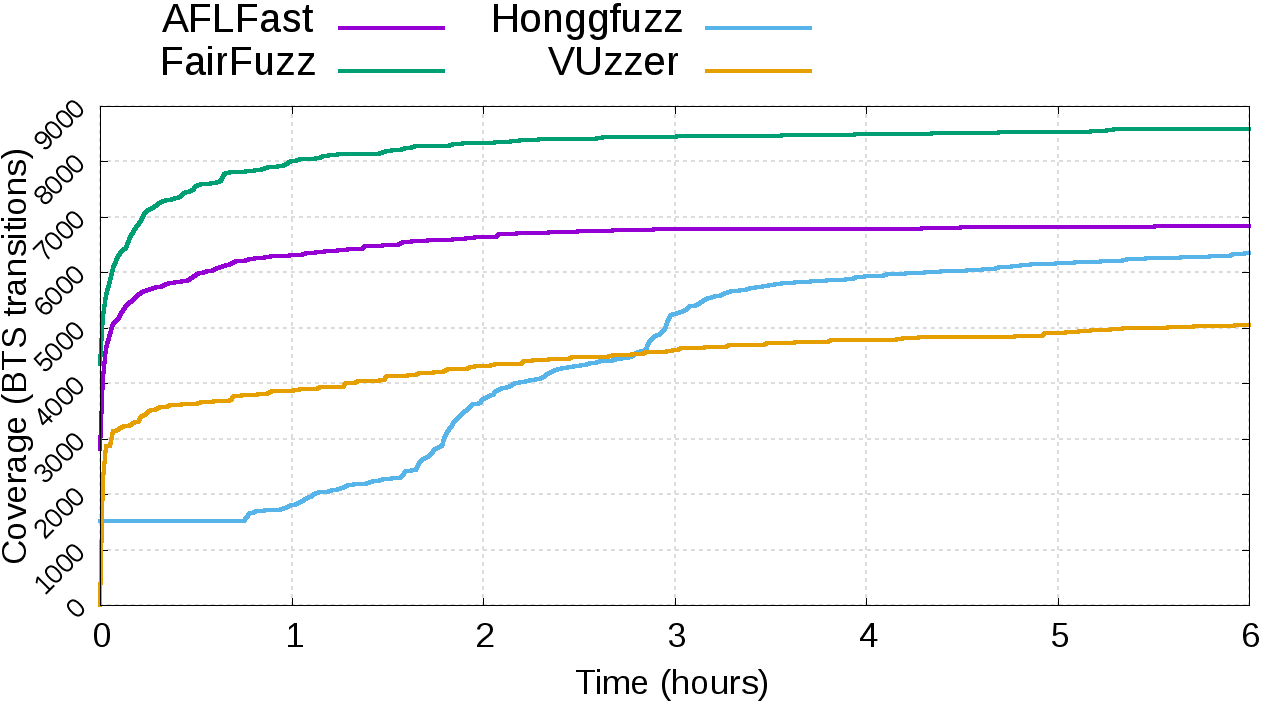
\includegraphics[width=.65\textwidth]{figures/mono-ming}
            \label{fig:eval-mono-ming}
        }
    \end{adjustbox}
    \caption{Mean coverage over time for single fuzzers.}
    \label{fig:eval-mono}
\end{figure}

To derive more robust and meaningful insights over these results, we employ the
Bayesian estimation model proposed in~\cite{kruschke2013bayesian}. This model
provides, among others, estimates of the posterior distributions of the means
and their differences of two given sets of observations.
\autoref{fig:djpeg-means} shows the distribution of the difference of means of
\honggfuzz\ against \aflfast\ and \fairfuzz\ for \djpeg. The figure also shows
the $95\%$ \ac{HDI}, which represents the interval of values onto which $95\%$
of the probability mass lies. \autoref{fig:djpeg-m-hongg-afl} clearly shows that
the \ac{HDI} lies completely above zero, meaning that with high credibility we
can say that \honggfuzz\ performs better than \aflfast\ over \djpeg.
Unfortunately the same conclusion cannot be made for the comparison of
\honggfuzz\ against \fairfuzz. \autoref{fig:djpeg-m-hongg-fair} shows that a
difference of means of zero lies on the \ac{HDI}; moreover an estimated $20.2\%$
of the probability mass lies below zero (\ie~in favor of \fairfuzz).

\begin{figure}[h]
    \centering%
    \subfloat[\honggfuzz\ vs.\ \aflfast]{%
        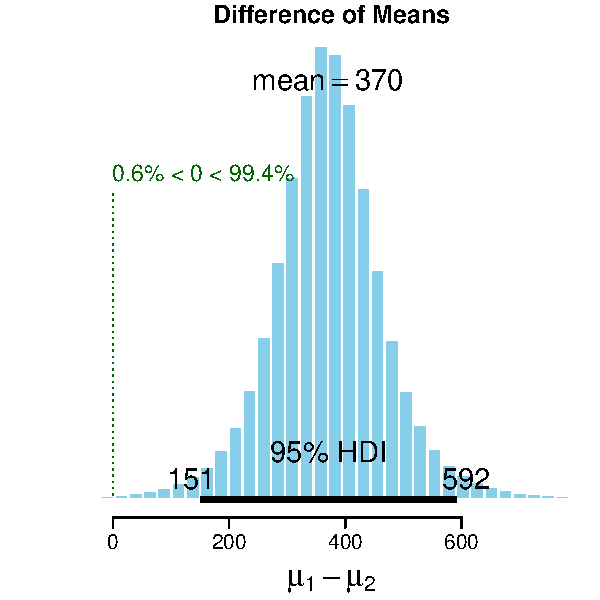
\includegraphics[width=.4\textwidth]{figures/cropped/djpeg-m-hongg-afl}
        \label{fig:djpeg-m-hongg-afl}
    }
    \subfloat[\honggfuzz\ vs.\ \fairfuzz]{%
        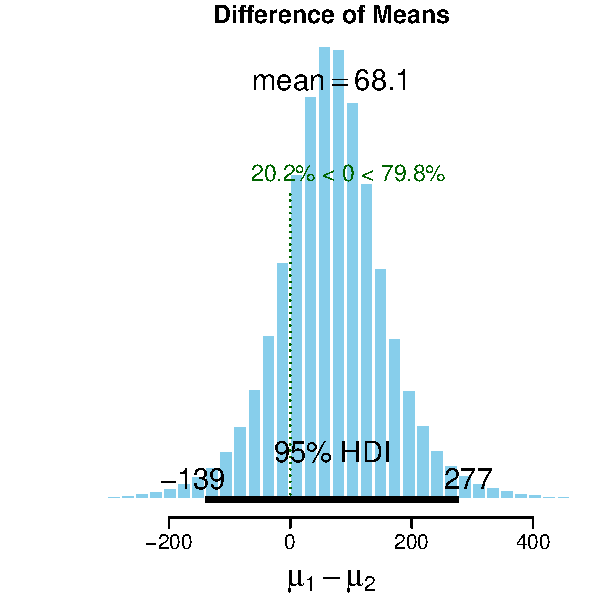
\includegraphics[width=.4\textwidth]{figures/cropped/djpeg-m-hongg-fair}
        \label{fig:djpeg-m-hongg-fair}
    }
    \caption{Single fuzzers: distribution of difference of means for \djpeg.}
    \label{fig:djpeg-means}
\end{figure}

\autoref{fig:objdump-means} shows the difference of means for \objdump. For both
the cases of \fairfuzz\ against \aflfast\ (\autoref{fig:objdump-m-fair-afl}) and
\fairfuzz\ against \honggfuzz\ (\autoref{fig:objdump-m-fair-hongg}) the results
strongly support the claim of \fairfuzz\ uncovering more basic block transitions
for \objdump.

\begin{figure}[h]
    \centering%
    \subfloat[\fairfuzz\ vs.\ \aflfast]{%
        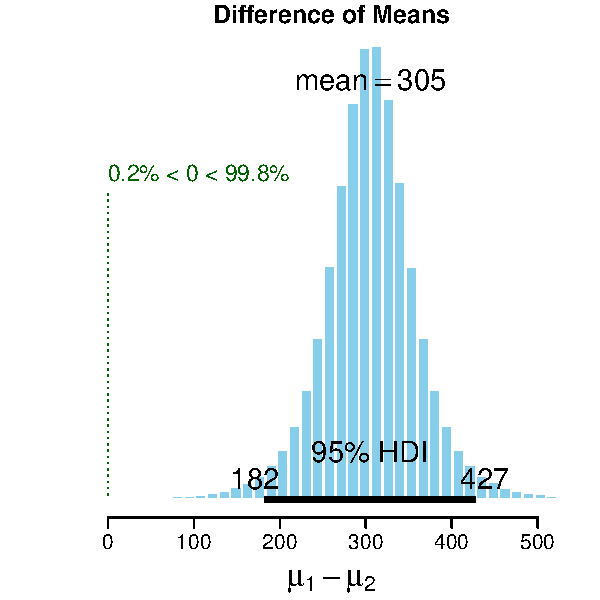
\includegraphics[width=.4\textwidth]{figures/cropped/objdump-m-fair-afl}
        \label{fig:objdump-m-fair-afl}
    }
    \subfloat[\fairfuzz\ vs.\ \honggfuzz]{%
        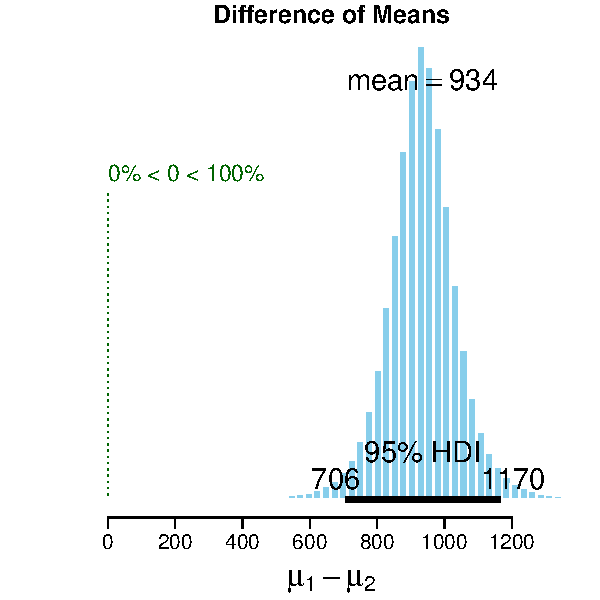
\includegraphics[width=.4\textwidth]{figures/cropped/objdump-m-fair-hongg}
        \label{fig:objdump-m-fair-hongg}
    }
    \caption{Single fuzzers: distribution of difference of means for \objdump.}
    \label{fig:objdump-means}
\end{figure}

\autoref{fig:tiff2pdf-means} shows the difference of means for \tiffpdf.
Unfortunately, as for \djpeg, we are not able to decisively confirm whether
\aflfast\ is better than \fairfuzz\ (\autoref{fig:tiff2pdf-m-afl-fair}). We can
be instead more certain affirming that \aflfast\ outperforms \honggfuzz\ for the
given \sut\ (\autoref{fig:tiff2pdf-m-afl-hongg}).

\begin{figure}[h]
    \centering%
    \subfloat[\aflfast\ vs.\ \fairfuzz]{%
        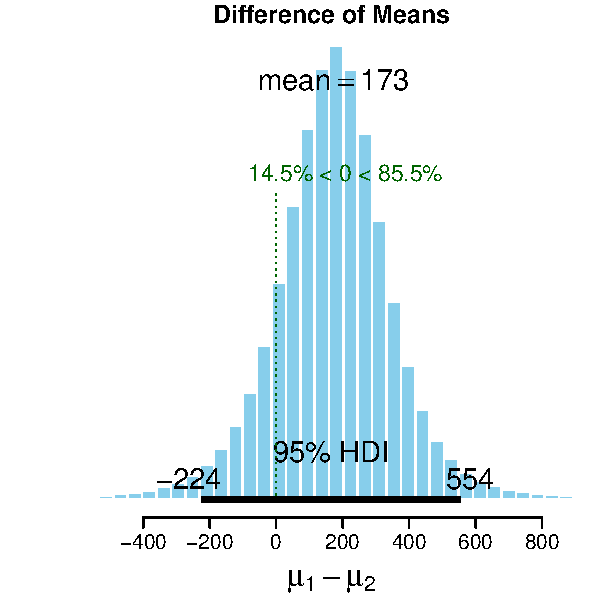
\includegraphics[width=.4\textwidth]{figures/cropped/tiff2pdf-m-afl-fair}
        \label{fig:tiff2pdf-m-afl-fair}
    }
    \subfloat[\aflfast\ vs.\ \honggfuzz]{%
        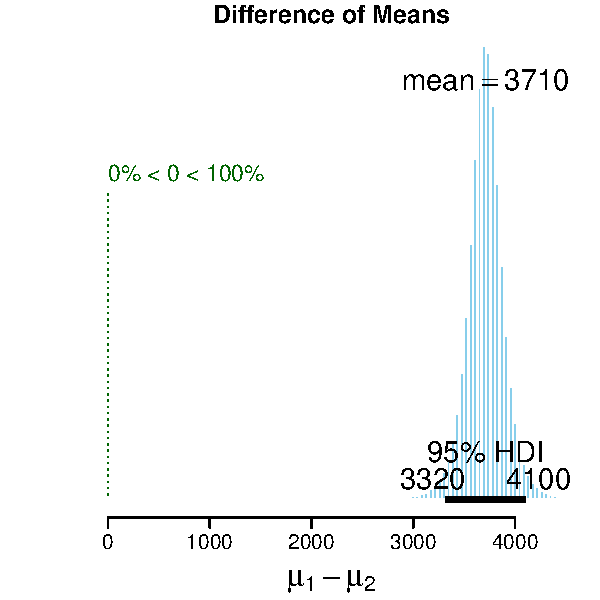
\includegraphics[width=.4\textwidth]{figures/cropped/tiff2pdf-m-afl-hongg}
        \label{fig:tiff2pdf-m-afl-hongg}
    }
    \caption{Single fuzzers: distribution of difference of means for \tiffpdf.}
    \label{fig:tiff2pdf-means}
\end{figure}

To validate differences among fuzzers even further, we compare, in
\autoref{tab:eval-mono-union}, the best single fuzzer with the result of taking
the union of coverage traces across all four fuzzers for each time step. The
table clearly shows that fuzzers uncover unique basic block transitions that are
not exposed by any other fuzzer (\ie~uncover disjoint sets of transitions) and
this contributes to reaching an higher final coverage consistently across all
examined programs.

\begin{table}[h]
    \centering%
    \begin{tabular}{l c l c}
        \textbf{\sut} & \multicolumn{2}{c}{\textbf{best single}} & \textbf{union} \\
        \bottomrule%
        \djpeg& $4112.8 \pm 39.5476$ & \honggfuzz& \hicell$4157.2 \pm 40.0495$ \\
        \objdump& $5067 \pm 62.6821$ & \fairfuzz& \hicell$5404.6 \pm 38.1997$ \\
        \tiffpdf& $8971.2 \pm 152.8626$ & \aflfast& \hicell$9695 \pm 129.7239$ \\
        \listswf& $8586.8 \pm 87.7451$ & \fairfuzz& \hicell$8916.6 \pm 83.8365$
    \end{tabular}
    \caption{Mean coverage with $95\%$ confidence intervals for best single
    fuzzer and union of coverage traces.}
    \label{tab:eval-mono-union}
\end{table}

To delve deeper into these values, we show the result of Bayesian estimation in
\autoref{fig:means-mono-union}. The $95\%$ \ac{HDI} falls above zero (\ie~in
favour of the union of fuzzers) for all considered programs except \djpeg, for
which the results are inconclusive.

\begin{figure}[h]
    \centering%
    \subfloat[\djpeg: Union vs.\ \honggfuzz]{%
        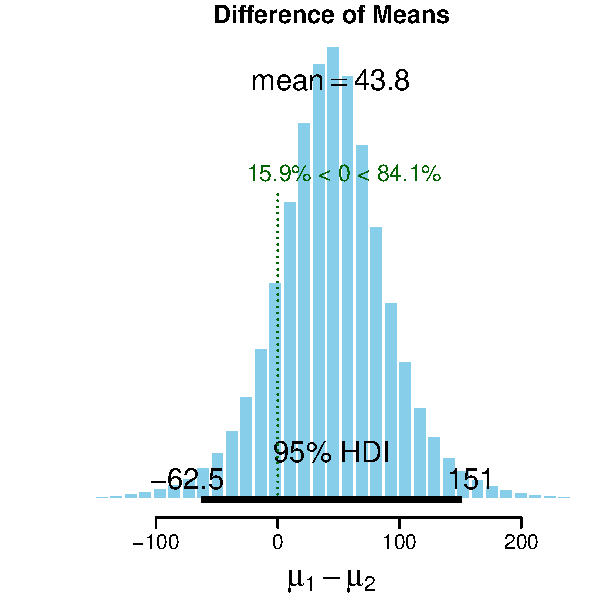
\includegraphics[width=.4\textwidth]{figures/cropped/djpeg-m-uni-hongg}
    }
    \subfloat[\objdump: Union vs.\ \fairfuzz]{%
        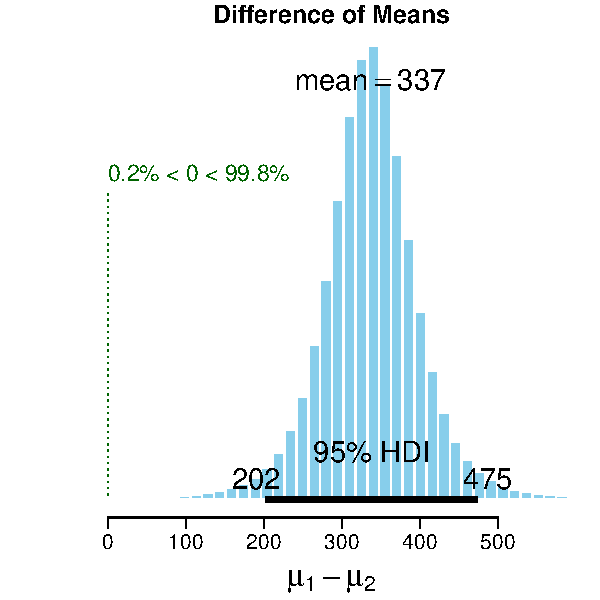
\includegraphics[width=.4\textwidth]{figures/cropped/objdump-m-uni-fair}
    }\\
    \subfloat[\tiffpdf: Union vs.\ \aflfast]{%
        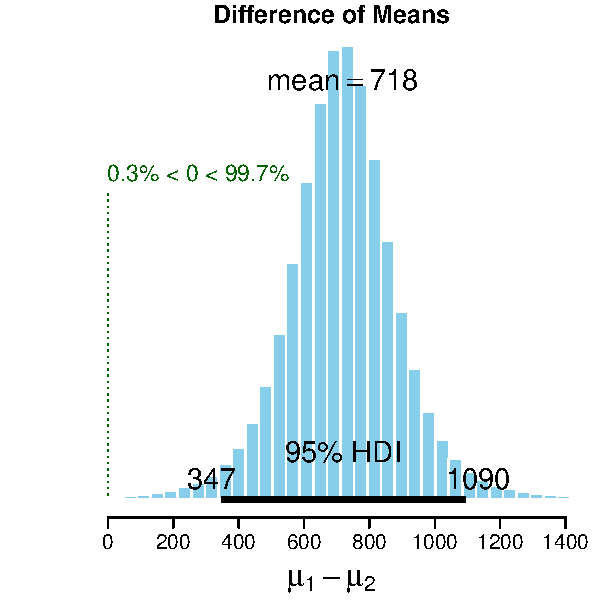
\includegraphics[width=.4\textwidth]{figures/cropped/tiff2pdf-m-uni-afl}
    }
    \subfloat[\listswf: Union vs.\ \fairfuzz]{%
        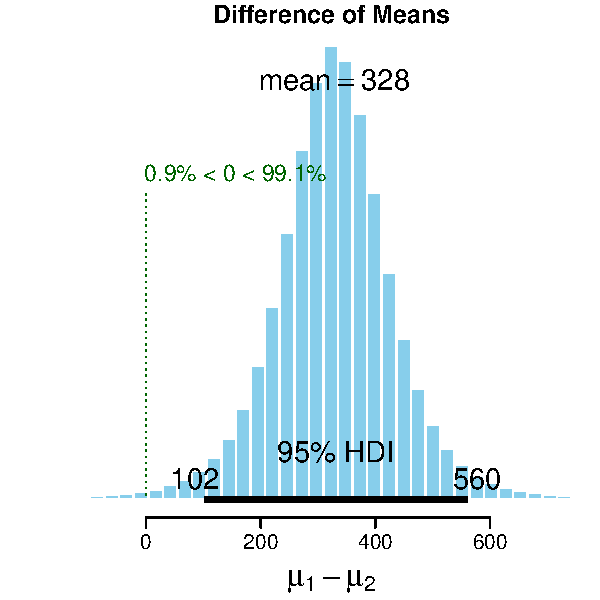
\includegraphics[width=.4\textwidth]{figures/cropped/ming-m-uni-fair}
    }
    \caption{Distribution of difference of means for union of fuzzers against
    the best single fuzzer.}
    \label{fig:means-mono-union}
\end{figure}

\section{Cooperative Fuzzing Evaluation}
\label{sec:eval-coop}

In this section we present an evaluation of the efficacy of cooperation. For
this purpose we compare the results of running the \ac{CFF} for $6$ hours with
the union of coverage from the four fuzzers running without cooperation, as we
have done in \autoref{sec:eval-mono}. To make the comparison fair, for the union
we take the maximum coverage after $6$ hours. We configured the \texttt{master}
to execute two distinct winning strategies: one selects the single fuzzer with
the highest metric reply; the other selects all fuzzers for which the metric
reply is greater than zero. In case of a draw, the pool of candidate winners is
randomly shuffled and the first one is selected. Recall from
\autoref{sec:driver-impl} that the metric is given by the number of undiscovered
branches exercised by the given input (the metric is the same for all drivers).
In this section we compare the results of running both strategies.

\begin{table}[h]
    \centering%
    \begin{tabular}{l c c c}
        \textbf{\sut} & \textbf{multi} & \textbf{single} & \textbf{union} \\
        \bottomrule%
        \djpeg& $4056.4 \pm 76.9499$ & \hicell$4078.4 \pm 85.6738$ & $4028.6 \pm 47.7396$ \\
        \objdump& $5414.6 \pm 224.121$ & \hicell$5529.6 \pm 338.651$ & $5035.6 \pm 54.5944$ \\
        \tiffpdf& \hicell$8765.6 \pm 183.682$ & $8577.6 \pm 99.2457$ & $8623.2 \pm 183.399$ \\
        \listswf& \hicell$9008.4 \pm 122.81$ & $8801.4 \pm 96.4045$ & $8916.6 \pm 83.8381$
    \end{tabular}
    \caption{Mean coverage with $95\%$ confidence intervals for winning
    strategies that select single or multiple winners and without cooperation.}
    \label{tab:eval-coop}
\end{table}

\autoref{tab:eval-coop} presents the final mean coverage with $95\%$ confidence
intervals. Looking only at the final mean we can see that one of the two
cooperative strategies outperforms the union of fuzzers for all programs, but
none of the two outperforms the other. Moreover for \djpeg\ and \objdump\ the
union of fuzzers seems to perform the worst while for \tiffpdf\ and \listswf\ it
is the single winner cooperative strategy to be outperformed. For \djpeg\ we see
that the differences are too small to be sensitive enough as is confirmed by
Bayesian estimation in \autoref{fig:best-djpeg-single-union} and
\autoref{fig:best-djpeg-single-multi}. By observing the mean coverage over time,
shown in \autoref{fig:eval-coop-djpeg}, we see that the union of fuzzers
struggles against both cooperative strategies for the first two hours, before
catching up.

\begin{figure}[h]
    \centering%
    \begin{adjustbox}{center}
        \subfloat[\djpeg]{%
            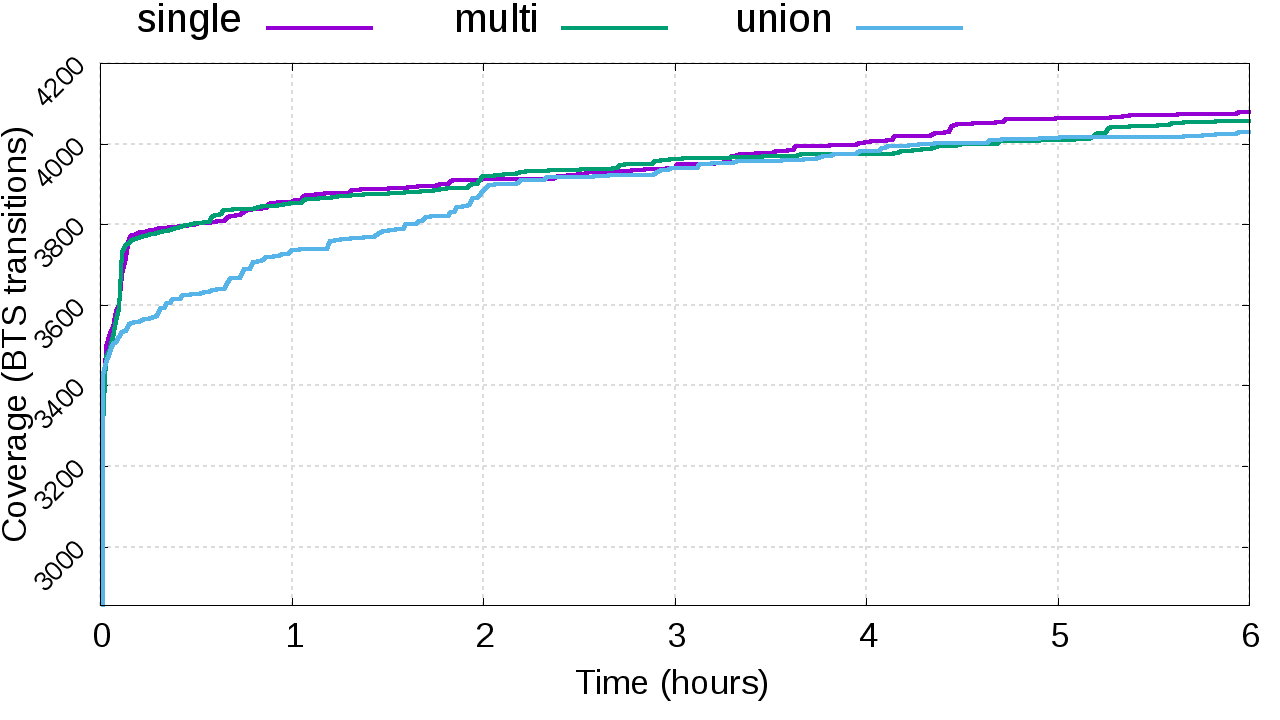
\includegraphics[width=.65\textwidth]{figures/vs-djpeg}
            \label{fig:eval-coop-djpeg}
        }
        \subfloat[\objdump]{%
            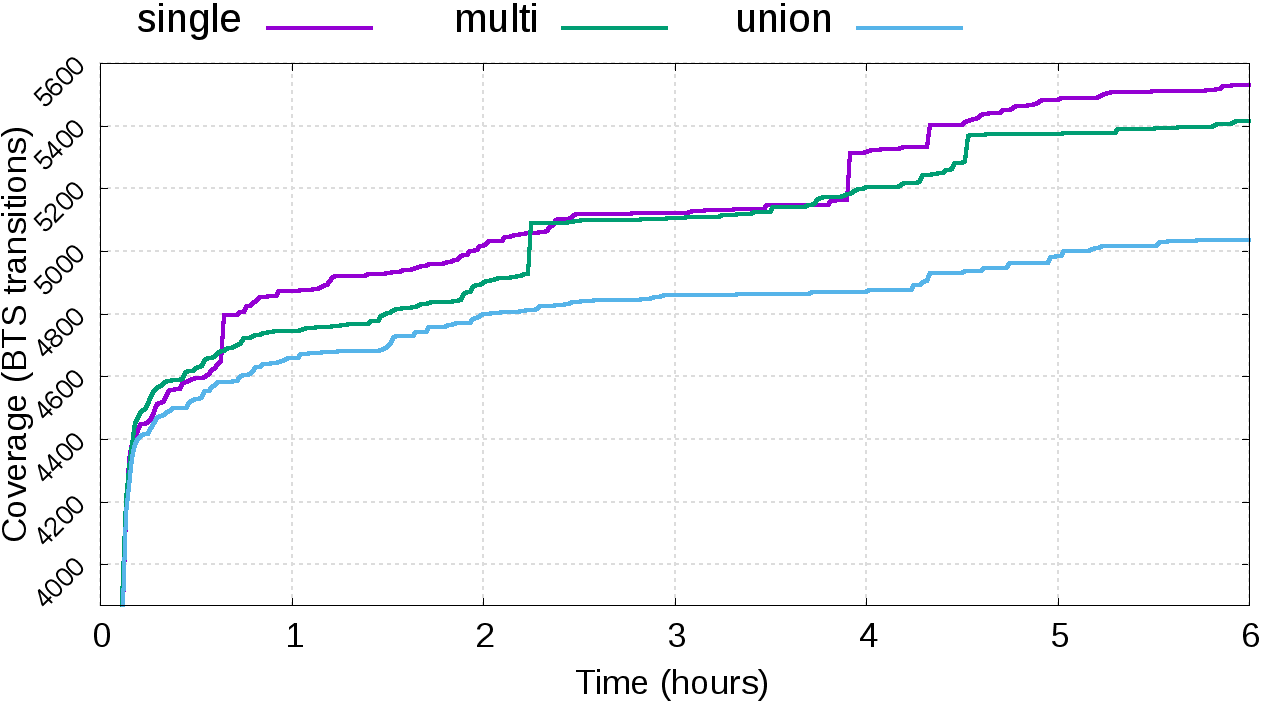
\includegraphics[width=.65\textwidth]{figures/vs-objdump}
            \label{fig:eval-coop-objdump}
        }
    \end{adjustbox}
    \begin{adjustbox}{center}
        \subfloat[\tiffpdf]{%
            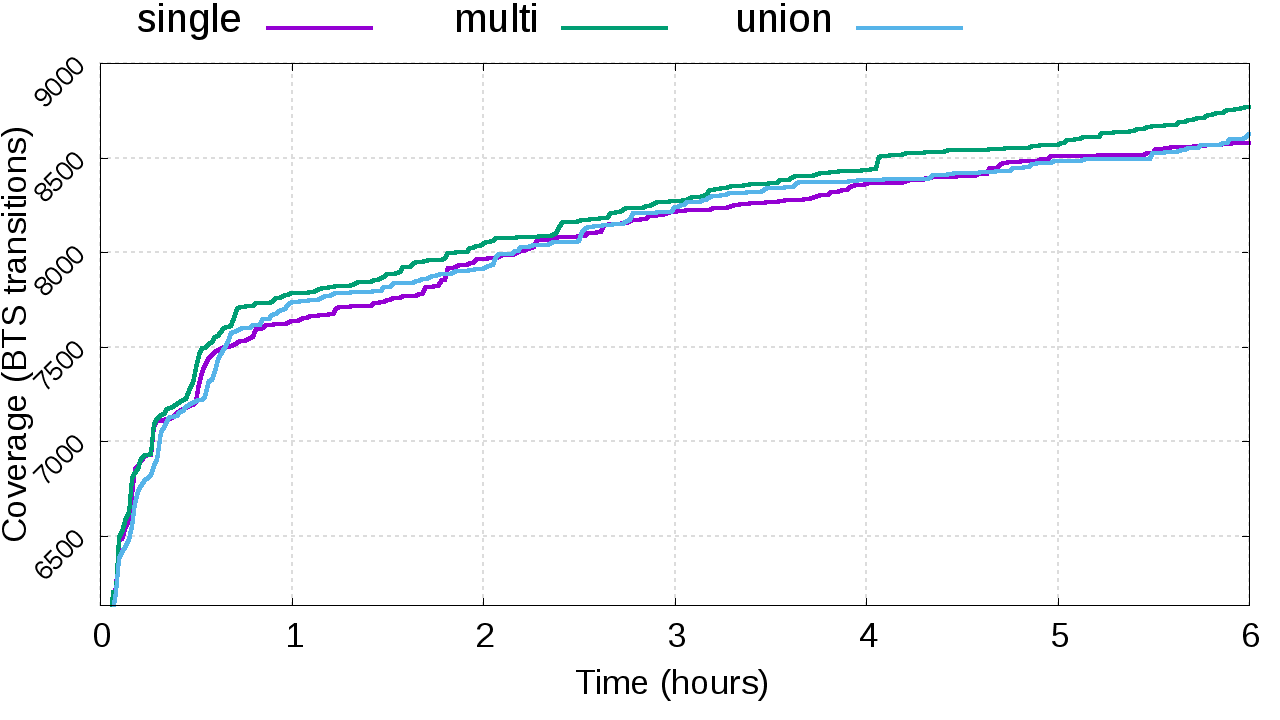
\includegraphics[width=.65\textwidth]{figures/vs-tiff2pdf}
            \label{fig:eval-coop-tiff2pdf}
        }
        \subfloat[\listswf]{%
            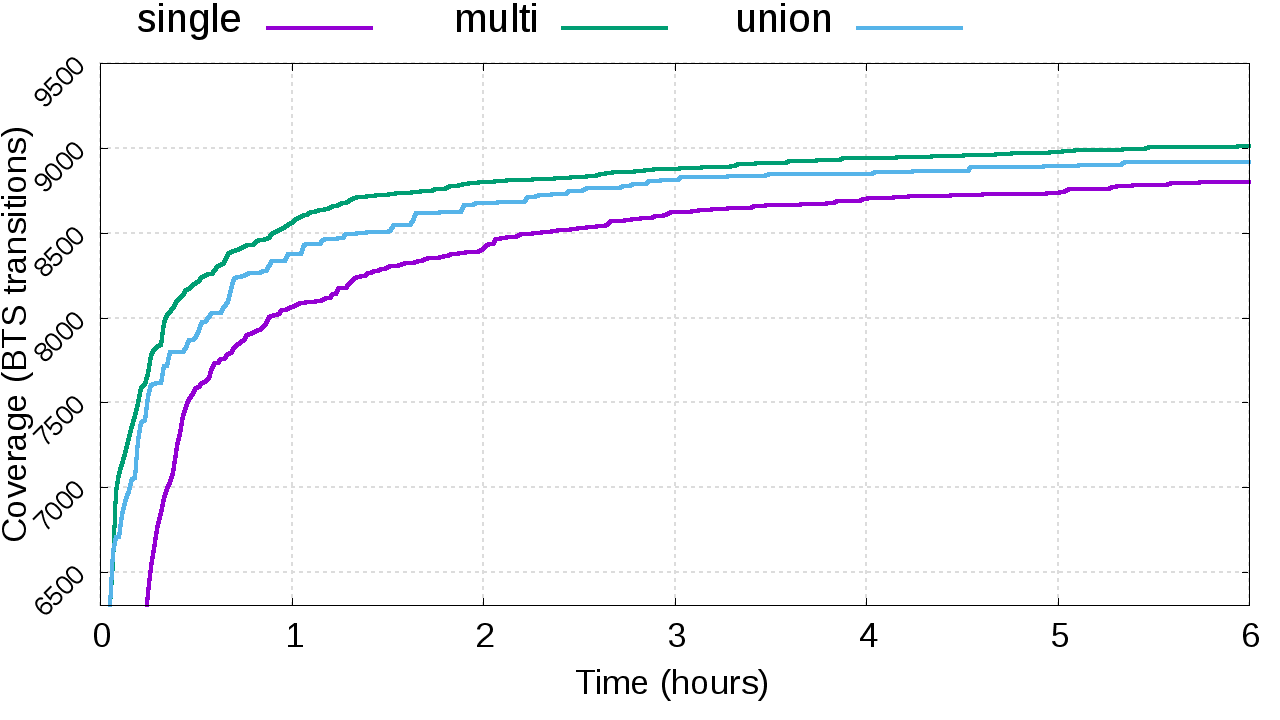
\includegraphics[width=.65\textwidth]{figures/vs-ming}
            \label{fig:eval-coop-ming}
        }
    \end{adjustbox}
    \caption{Mean coverage over time for two cooperative strategies and union of
    fuzzers.}
    \label{fig:eval-coop}
\end{figure}

The mean final coverage for cooperative strategies may seem to be better than
the union of fuzzers for \objdump\ (\autoref{fig:eval-coop-objdump}) as both
means are higher and their confidence interval do not overlap with the one for
the union. Unfortunately Bayesian estimation does not support these conclusions
with high credibility (\ie~the \ac{HDI} for the difference of means includes
zero) as shown in \autoref{fig:best-objdump-single-union} for the single winner
strategy against the union of fuzzers and \autoref{fig:best-objdump-multi-union}
for the multiple winners strategy against the union. In both cases, however,
respectively $95.4\%$ and $96.7\%$ of the credible values of the difference of
means are greater than zero (\ie~in favour of the cooperative strategy).

In the case of \tiffpdf\ and \listswf\ we are presented with similar results as
in both cases the single winner strategy is outperformed by the other
cooperative strategy and the union of fuzzers.
\autoref{fig:best-tiff2pdf-multi-union} and
\autoref{fig:best-tiff2pdf-multi-single} show the results of Bayesian estimation
on \tiffpdf\ for the multiple winners strategy against the union and the single
winner strategy respectively; either case provides with means to say with an
high degree of certainty that the multiple winners strategy performs better than
the other. The coverage over time presented in \autoref{fig:eval-coop-tiff2pdf}
suggests one more thing: as time progresses, the distance between the multiple
winners strategy and the other two seems to increase; an evaluation over a
period of time longer than $6$ hours might reduce the variability of final
coverage and yield more conclusive results. Moreover we note how none of the
curves on the graph seem to end with a small or zero trend (\ie~none seem close
to convergence), suggesting that more time might reveal more basic block
transitions and possibly a more credible difference of means.

For \listswf, yet again, Bayesian estimation cannot provide us with enough
confidence to say that the multiple winners strategy uncovers more basic block
transitions than the union of fuzzers, as shown in
\autoref{fig:best-ming-multi-union}. Running the analysis to compare the results
of the two cooperative strategies yields uncertainty in confirming that
selecting multiple winners uncovers more basic block transitions than selecting
a single one; this is shown in \autoref{fig:best-ming-multi-single} where we see
that the \ac{HDI} includes zero and $94\%$ of the credible values are above
zero.

\section{Crash Analysis}
\label{sec:eval-crashes}

This section presents our findings regarding crashes based on the experiments
already described in \autoref{sec:eval-coop}. In the following we compare the
union of fuzzers and two cooperative strategies; in figures, ``mono'' (colour
red) refers to the union, ``multi'' (green) and ``single'' (blue) refer to the
multiple and single winner strategies respectively.

Unfortunately we were able to find crashes only in \listswf; when discussing
results, the remaining of the section does not refer to the \sut\ explicitly as
there is only one to consider for this analysis.

Before presenting the results, we ought to define some terminology and the
process that we used to obtain the final data. A \emph{unique crash} is an input
that causes a crash in the \sut\ through a unique path. Each of the fuzzers we
used in our experiments already track unique crashes, we developed some
additional scripts to post-process the data and aggregate results of the five
rounds we ran for each experiment. In particular, for each round of an
experiment we collect all unique crashes from the fuzzer's folder and run the
\sut\ with the given file (we also disable \ac{ASLR} and limit the address space
appropriately). If the program terminates with a crash or timeouts (the time
limit is taken from the respective fuzzer's parameter), we run the GDB utility
\texttt{exploitable}~\cite{foote2013cert} and \texttt{backtrace} command and
store the output into a file. The \emph{stack hash} computed by
\texttt{exploitable}, which is the hash of the last five calls on the stack, is
used to identify a unique crash. Then, for each experiment, we aggregate the
results of the rounds into a single file that contains the elapsed time at which
the crash was discovered and the stack hash; moreover, we do not remove
duplicates.

\autoref{tab:crashes} shows the number of \emph{distinct} unique crashes found
across five rounds of each experiment, alongside the number of distinct crashes
that were found by one experiment and not by the other.

\begin{table}[h]
    \centering%
    \begin{tabular}{l c c c c}
        & \textbf{Unique crashes} & \textbf{Vs.\ single} &
            \textbf{Vs.\ multi} & \textbf{Vs.\ union} \\
        \bottomrule%
        \textbf{union} & $75$ & $21$ & $13$ & \\
        \hline%
        \textbf{multi} & $98$ & $44$ & & $36$ \\
        \hline%
        \textbf{single} & $63$ & & $9$ & $9$
    \end{tabular}
    \caption{Distinct unique crashes and amount discovered by one and not
    discovered by another.}
    \label{tab:crashes}
\end{table}

\autoref{fig:unique-crashes} presents the evolution over time of the unique
crashes aggregated from the five rounds; in particular,
\autoref{fig:crashes-count} shows the cumulative count of unique crashes, while
\autoref{fig:crashes-density} shows their density.

\begin{figure}[h]
    \centering%
    \subfloat[Cumulative count of unique crashes.]{%
        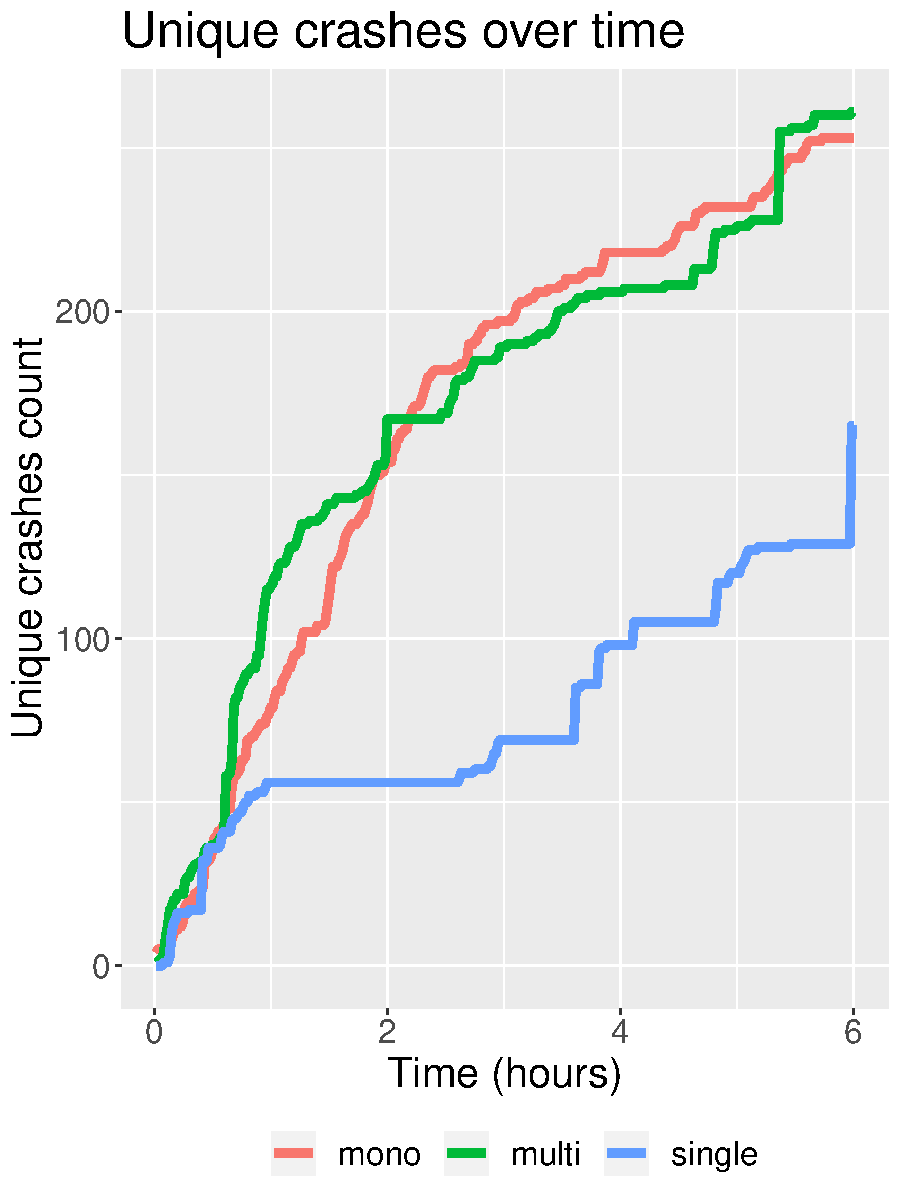
\includegraphics[width=.5\textwidth]{figures/cropped/crashes-count-all}
        \label{fig:crashes-count}
    }
    \subfloat[Density of unique crashes.]{%
        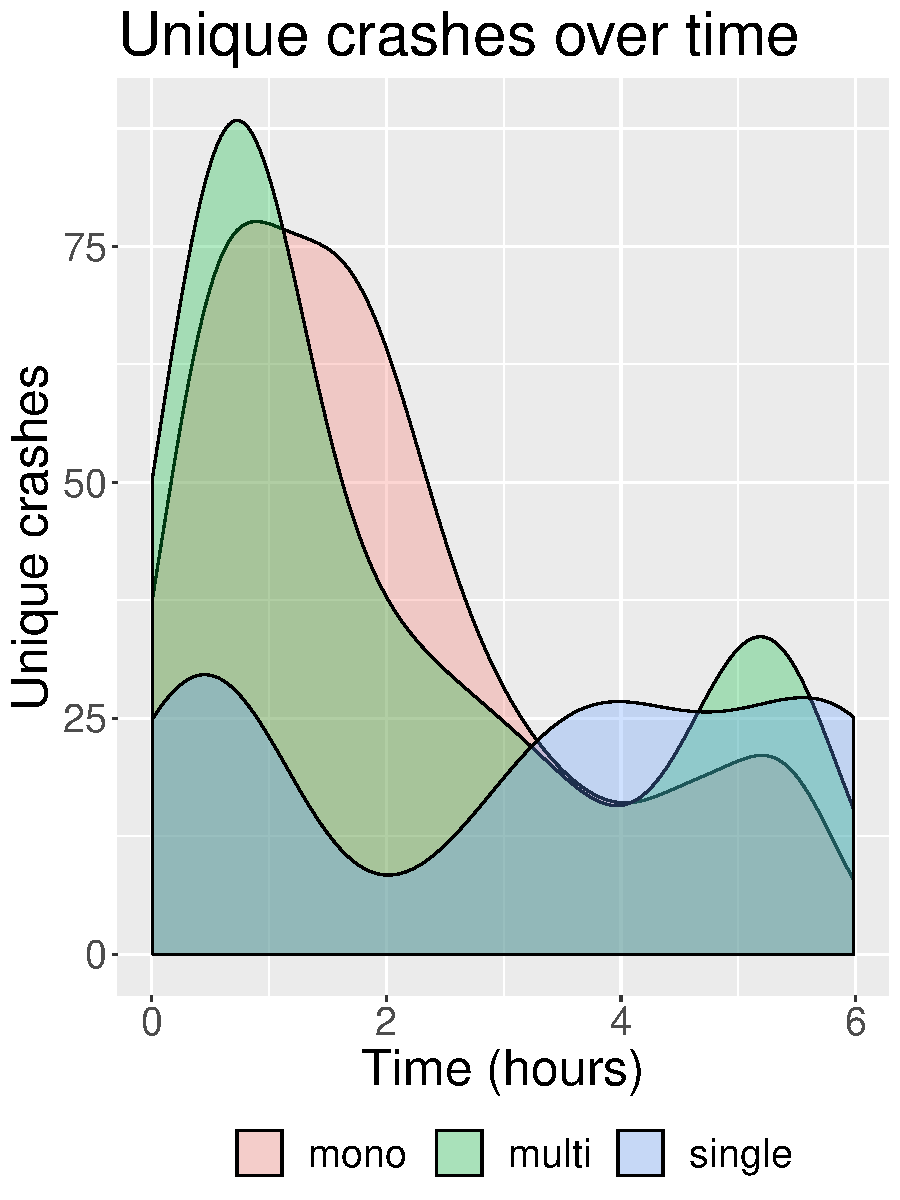
\includegraphics[width=.5\textwidth]{figures/cropped/crashes-all}
        \label{fig:crashes-density}
    }
    \caption{Unique crashes over time for \listswf.}
    \label{fig:unique-crashes}
\end{figure}

With regards to the cumulative count, we see that not only the multiple winners
strategy finds more distinct unique crashes (\ie~$98$ against $75$), but also
the number of unique crashes itself it higher. Moreover, we see that the number
of unique crashes for multiple winners is briefly taken over by that of the
union of fuzzers, before becoming the highest again toward the end of the runs;
this is also highlighted by the strongly bi-modal nature of the density.

\autoref{fig:unique-crashes-inter} presents a subdivision of the results already
presented in \autoref{fig:crashes-density}: \autoref{fig:unique-crashes-common}
shows the density of unique crashes only for those that fall in the intersection
among all three experiments; \autoref{fig:unique-crashes-uncommon} shows the
density for those that do not fall in the intersection.

\begin{figure}[h]
    \centering%
    \subfloat[Common unique crashes.]{%
        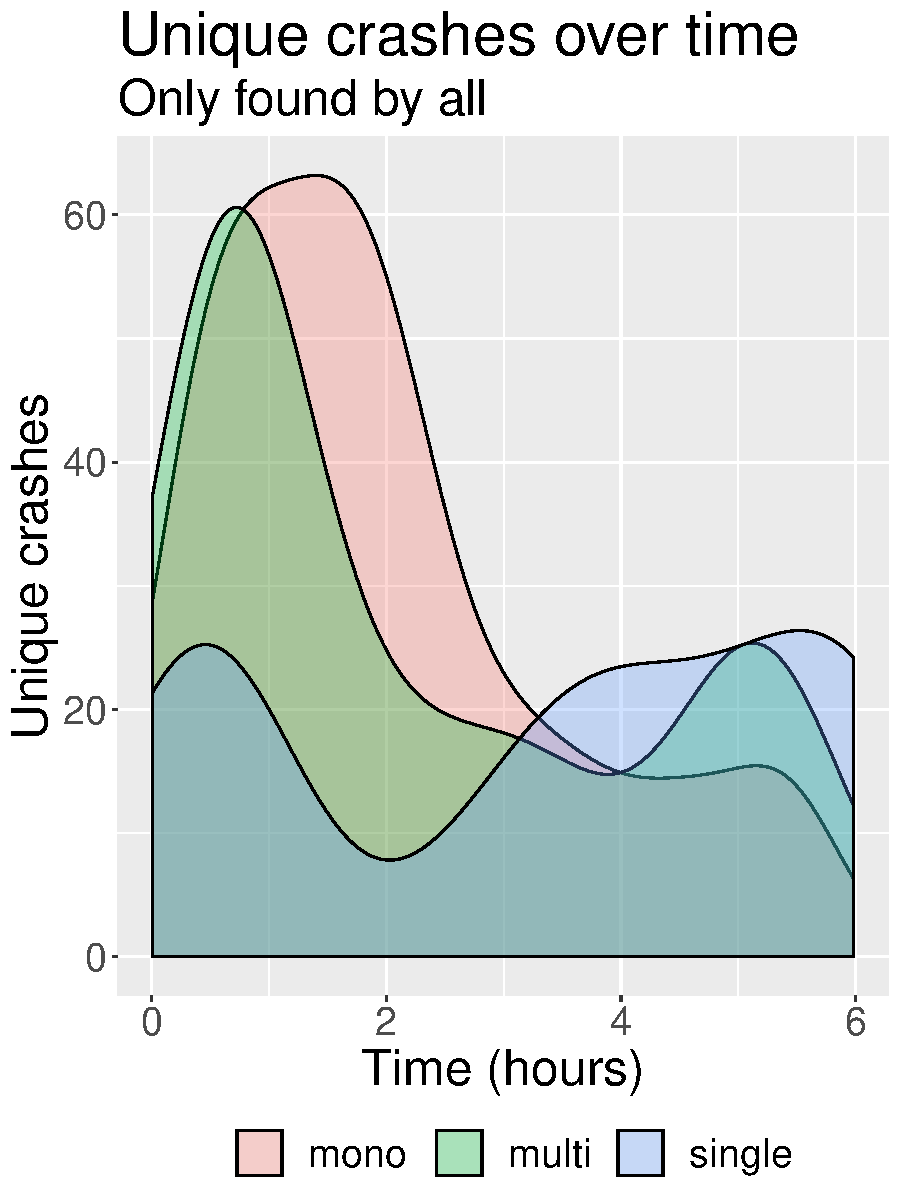
\includegraphics[width=.5\textwidth]{figures/cropped/crashes-intersect}
        \label{fig:unique-crashes-common}
    }
    \subfloat[Uncommon unique crashes.]{%
        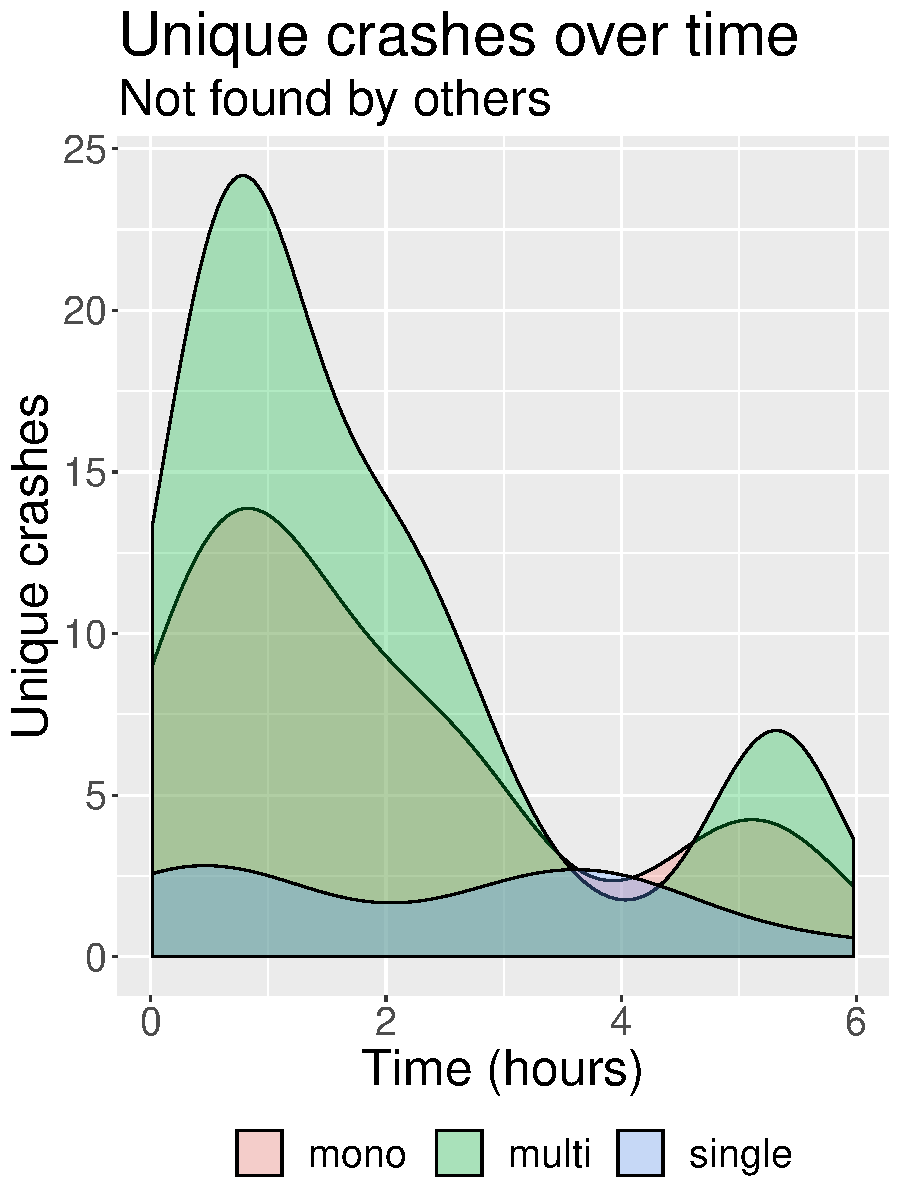
\includegraphics[width=.5\textwidth]{figures/cropped/crashes-not-intersect}
        \label{fig:unique-crashes-uncommon}
    }
    \caption{Density of unique crashes over time for \listswf, divided in
    intersection of hashes and not in the intersection.}
    \label{fig:unique-crashes-inter}
\end{figure}

From the figure, we see that for the intersection of crashes, the union of
fuzzers produces the most amount and, with the help of the density of the
remaining, we see that the multiple winners strategy's effort is spend producing
more crashes that are not found by the other experiments.

\subsection{Known Vulnerabilities}

For each of the unique crashes, we manually investigated the nature of the crash
and tried to link it to a known vulnerability with an assigned \ac{CVE}
identifier; note that multiple unique crashes may be caused by the same bug. We
found exclusively memory access violations caused by unchecked heap memory
allocations or reallocations, an example of which is given in \autoref{lst:cve}.
We were able to link six (of the over $25$ found) to a \ac{CVE}; for those we
report on the time of discovery in \autoref{fig:cves}.

\begin{lstlisting}[caption={Unchecked memory allocation in
                            \texttt{util/read.c:222} causing CVE-2017-7582.},
                   label=lst:cve, float=h, basicstyle=\ttfamily\footnotesize]
char *readBytes(FILE *f,int size)
{
  int i;
  char *buf;

  buf = (char *)malloc(sizeof(char)*size);

  for(i=0;i<size;i++)
  {
    buf[i]=(char)readUInt8(f);
  }

  return buf;
}
\end{lstlisting}

We see that all \acp{CVE} found by the union of fuzzers have been found by the
multiple winners strategy; moreover all but one are found on average before the
union does. The multiple winners strategy finds also two \acp{CVE} that are not
discovered by the union of fuzzers.

\begin{figure}[t]
    \centering%
    \subfloat{%
        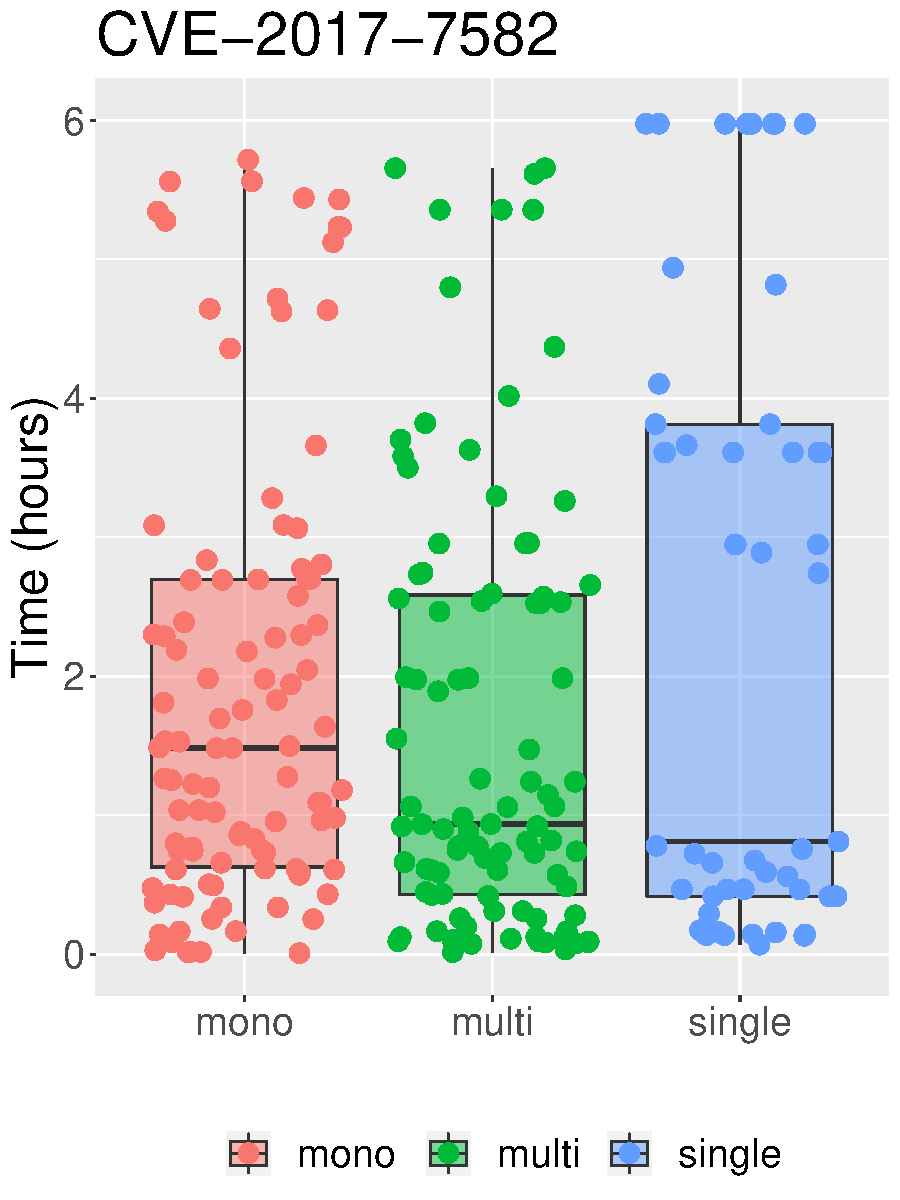
\includegraphics[width=.45\textwidth]{figures/cropped/cve-2017-7582}
    }
    \subfloat{%
        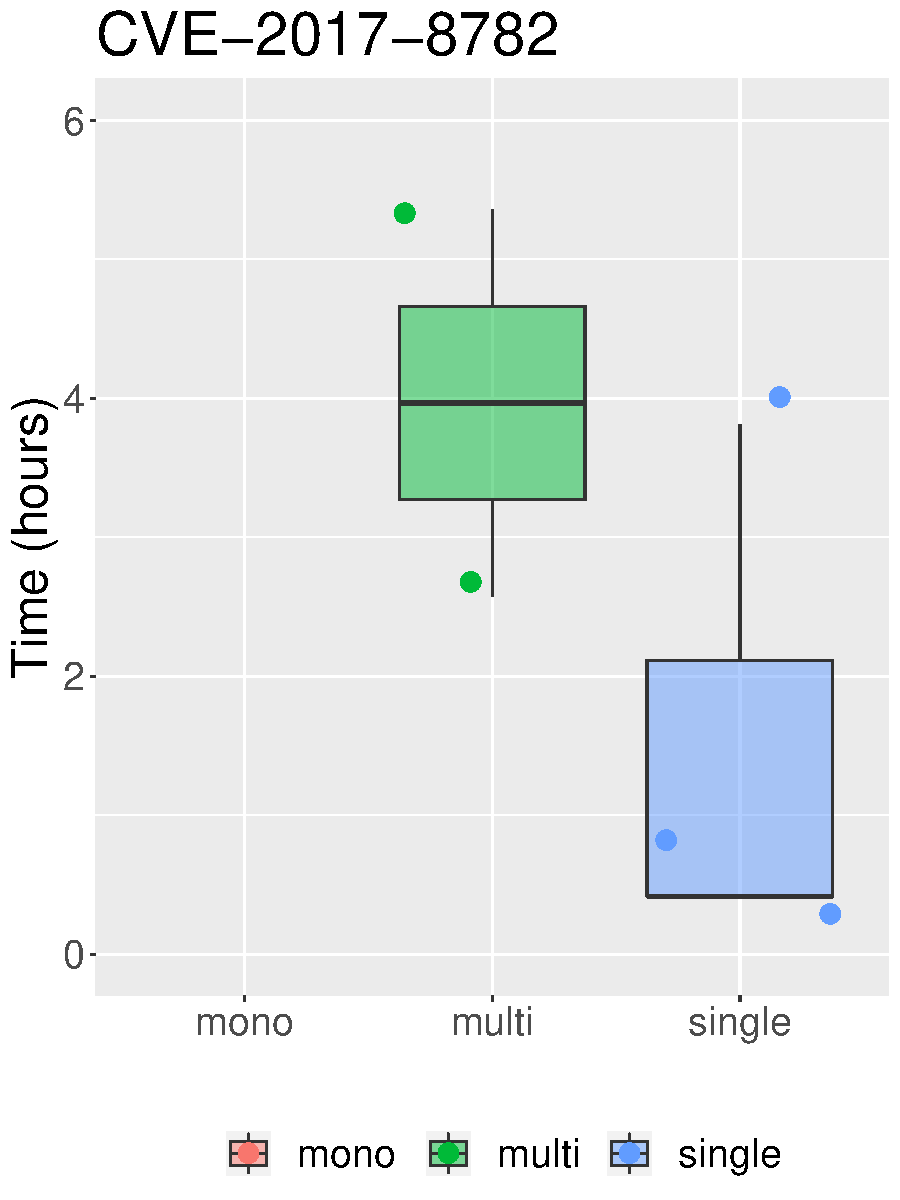
\includegraphics[width=.45\textwidth]{figures/cropped/cve-2017-8782}
    }\\
    \subfloat{%
        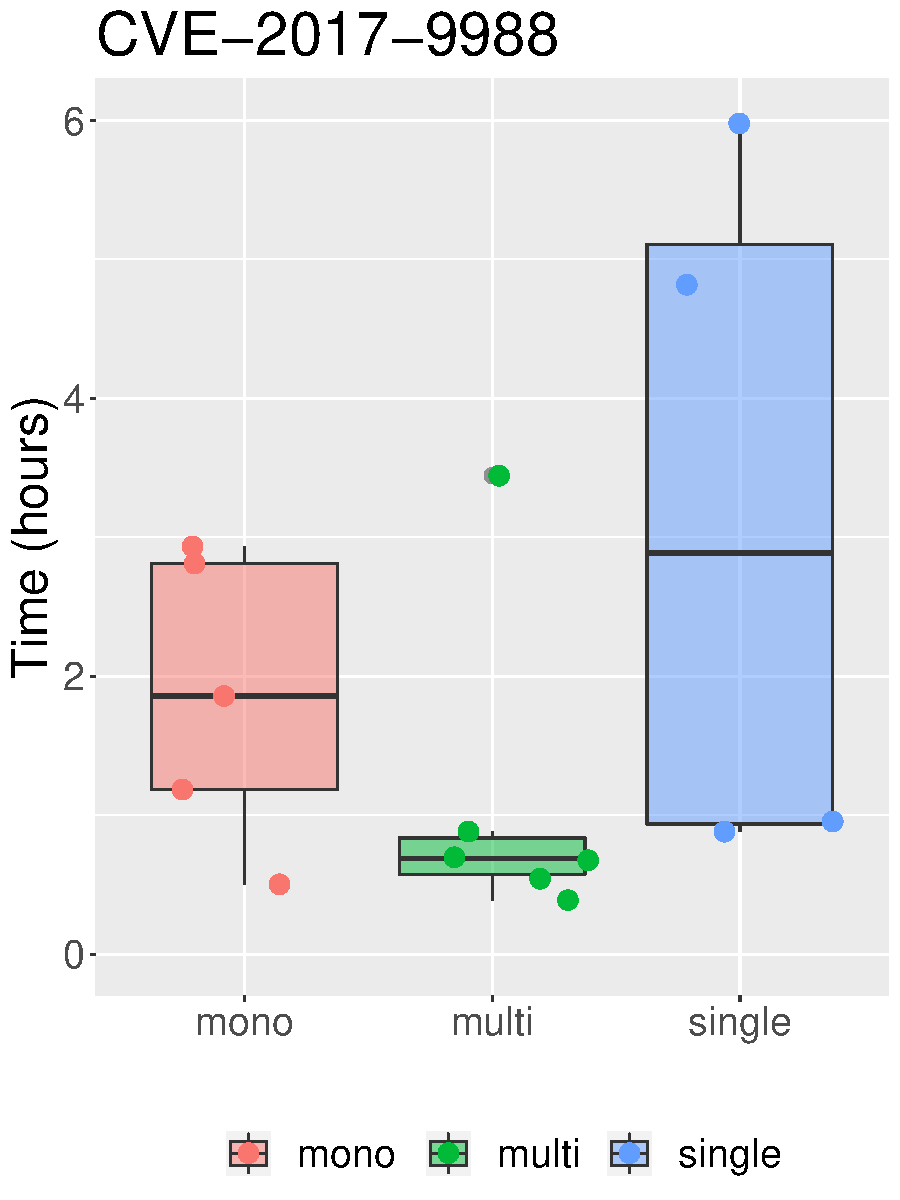
\includegraphics[width=.45\textwidth]{figures/cropped/cve-2017-9988}
    }
    \subfloat{%
        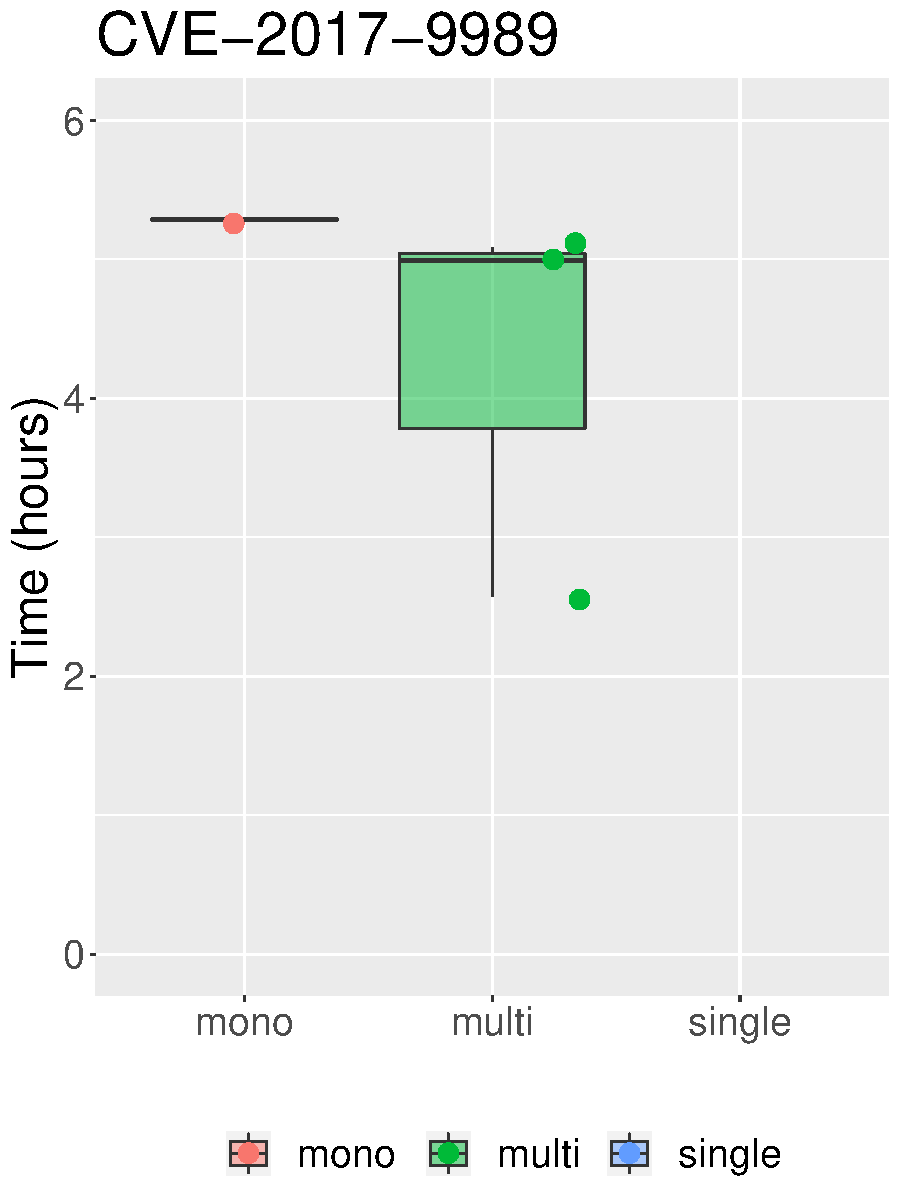
\includegraphics[width=.45\textwidth]{figures/cropped/cve-2017-9989}
    }\\
    \subfloat{%
        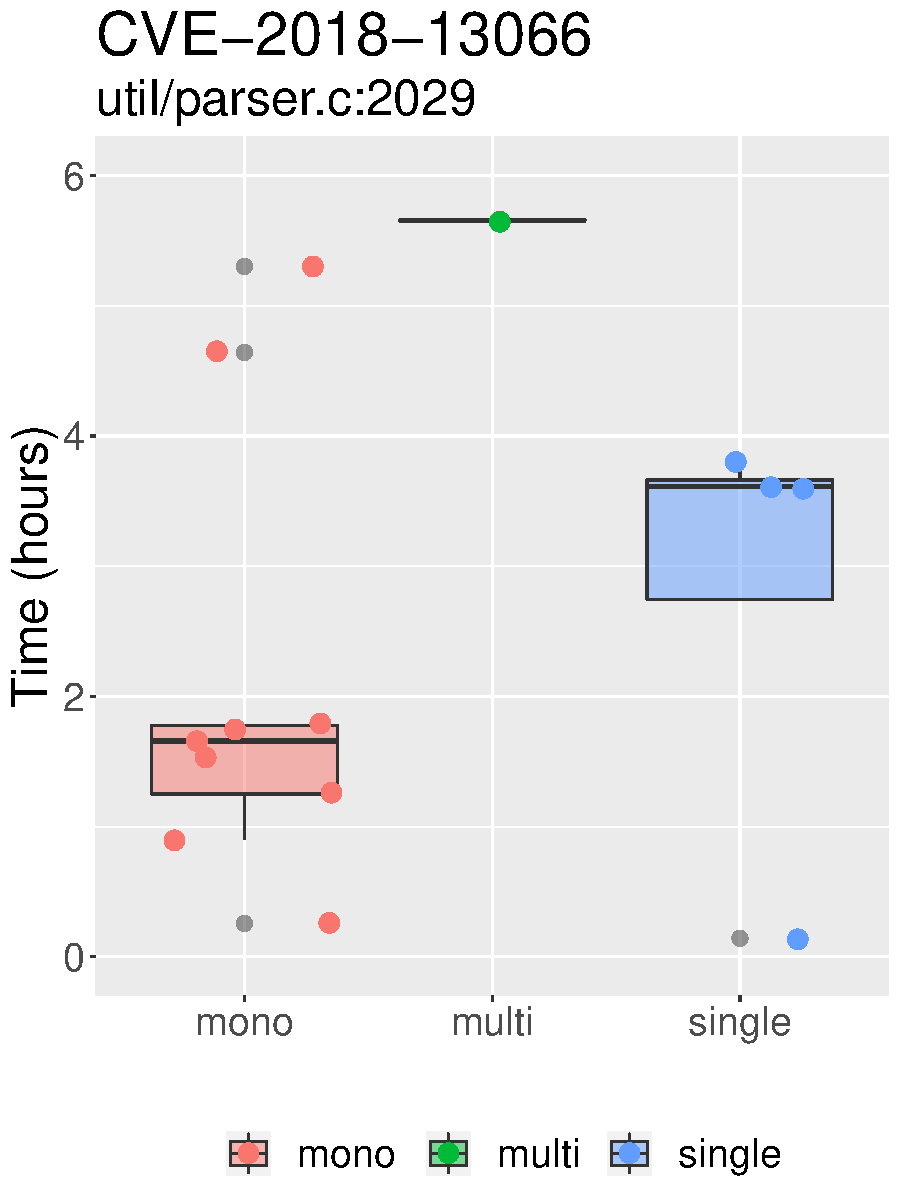
\includegraphics[width=.45\textwidth]{figures/cropped/cve-2018-13066-parser-2029}
    }
    \subfloat{%
        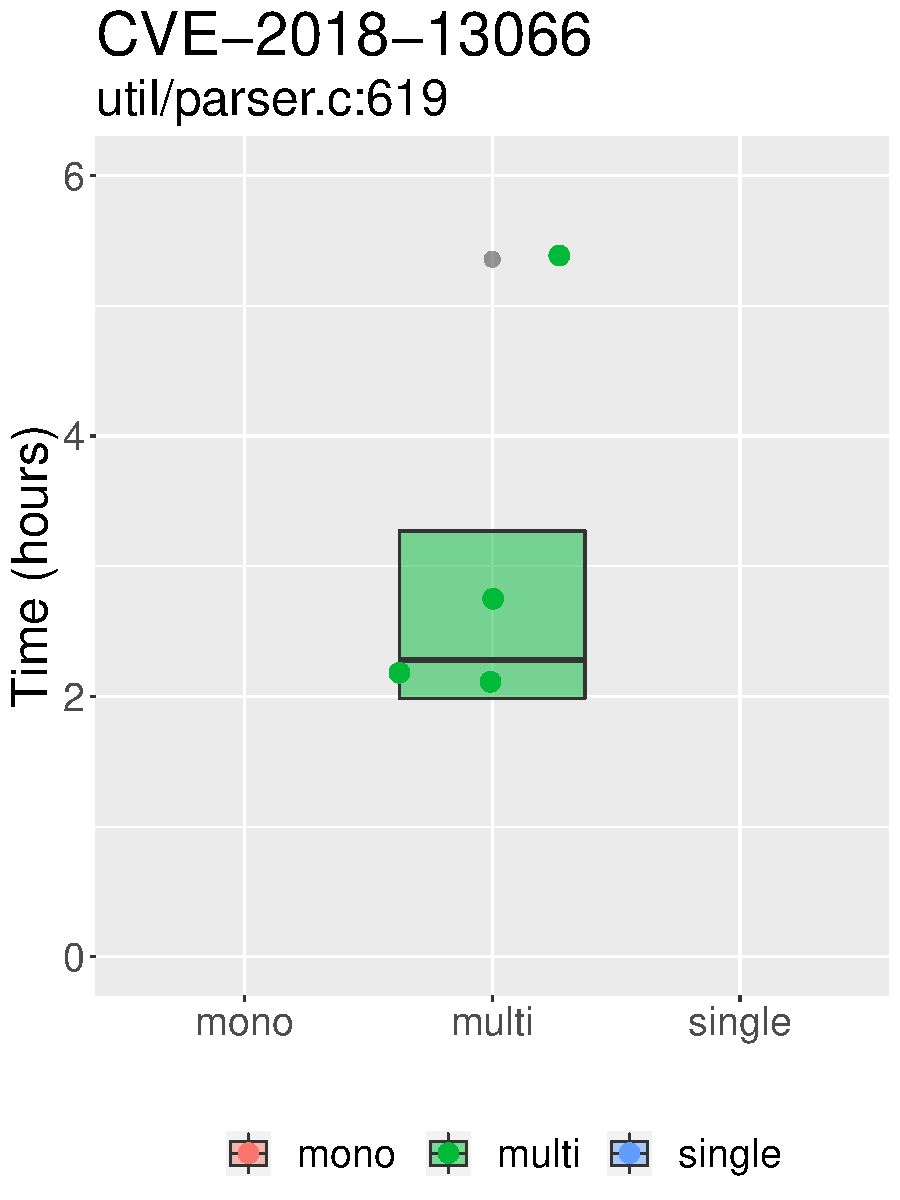
\includegraphics[width=.45\textwidth]{figures/cropped/cve-2018-13066-parser-619}
    }
    \caption{Bugs with assigned \acs{CVE} identifier found in \listswf.}
    \label{fig:cves}
\end{figure}


